\documentclass[11pt]{article}

\usepackage[a4paper,margin=1in]{geometry}
\usepackage[T1]{fontenc}
\usepackage[utf8]{inputenc}
\usepackage{lmodern}
\usepackage{microtype}
\usepackage{amsmath,amssymb,amsthm,mathtools}
\usepackage{booktabs}
\usepackage{graphicx}
\usepackage{float}
\usepackage{placeins}
\usepackage{enumitem}
\usepackage[numbers,sort&compress]{natbib}
\usepackage{xcolor}
\usepackage{xurl}
\usepackage[colorlinks=true,linkcolor=blue!55!black,citecolor=blue!55!black,urlcolor=blue!55!black]{hyperref}
\usepackage[nameinlink,noabbrev]{cleveref}

\setlength{\parindent}{1.4em}
\setlength{\parskip}{0.15em}
\setlist{itemsep=0.25em,topsep=0.35em}

\newtheorem{theorem}{Theorem}[section]
\newtheorem{proposition}[theorem]{Proposition}
\newtheorem{lemma}[theorem]{Lemma}
\newtheorem{corollary}[theorem]{Corollary}
\theoremstyle{definition}
\newtheorem{definition}[theorem]{Definition}
\theoremstyle{remark}
\newtheorem{remark}[theorem]{Remark}

\newcommand{\R}{\mathbb R}
\newcommand{\C}{\mathbb C}
\newcommand{\uc}{u_{\mathrm c}}
\newcommand{\Id}{\mathrm I}
\newcommand{\cK}{\mathcal K}
\newcommand{\cT}{\mathcal T}
\newcommand{\cR}{\mathcal R}
\newcommand{\cB}{\mathcal B}
\newcommand{\cC}{\mathcal C}
\newcommand{\cE}{\mathcal E}
\newcommand{\cH}{\mathcal H}
\newcommand{\cP}{\mathcal P}
\newcommand{\spec}{\operatorname{spec}}
\newcommand{\spr}{\operatorname{spr}}

\title{\textbf{Sector-Resolved Critical-Branch Returns}\
\textbf{at a Quadratic Band-Merging Map:}\\[0.35em]
\large Exact Two-Channel Factorization, a Dark Antisymmetric Mode,\\
and a Conditional Cubic-Phase Law}
\author{Liang Wang\\
\small School of Artificial Intelligence and Automation,\\[-0.2em]
\small Huazhong University of Science and Technology, Wuhan 430074, P.R. China\\
\small \texttt{wangliang.f@gmail.com}}
\date{July 2026}

\begin{document}

\maketitle

\begin{abstract}
At the first algebraic band-merging parameter of
$f_u(x)=1-u x^2$, the positive Gaussian return through both critical
preimages has a principal radius near $0.79$, whereas a single branch and
the parity-extracted physical bulk edge lie near $0.756$ at the smallest
computed noise.  The omitted branch is therefore not a small complement.
This paper asks whether a branch phase can supply the missing finite-channel
structure without confusing a time lift with the physical spectrum.

Let $\cC$ carry the endpoint packet into the direct sum of the left and
right critical windows, let $\cE$ return that branch space to the endpoint,
and put $J_\theta=\operatorname{diag}(1,e^{i\theta})$.  We prove the exact
factorization
\[
 \cR(\theta)=\cE J_\theta\cC
 =\cR_-+e^{i\theta}\cR_+,
 \qquad
 \cB(\theta)=J_\theta\cC\cE,
\]
and the Sylvester identity
\[
 \det(\Id-z\cR(\theta))
 =\det(\Id-z\cB(\theta)).
\]
Thus endpoint and branch formulations have the same nonzero spectrum; the
two-channel reduction is not a second spectral ansatz.

If the branch monodromy closes on one profile per branch and has rank one,
its only nonzero eigenvalue is
$\eta_-+e^{i\theta}\eta_+$.  Exact branch equivalence makes the unweighted
channel bright on the symmetric vector and dark on the antisymmetric vector.
Among unit-modulus relative weights, the requirement that the combined
return retain one-branch modulus then forces
$\theta=\pm2\pi/3$.  This cubic-phase law is conditional.  We also prove
that radial data alone cannot identify it: the half-weighted positive sum
$(\cR_-+\cR_+)/2$ has the same leading modulus in the symmetric rank-one
limit.  Moreover, a discrete period-$k$ Floquet sector contains the cubic
phase only when $3$ divides $k$.

Seven-noise computations show that a two-profile compression recovers the
full two-branch bright return while its dark/bright eigenvalue ratio falls to
$1.45\times10^{-5}$ at $\sigma=10^{-4}$.  At that noise, the phase preserving
one-branch modulus is $0.665704\pi$, the phase matching the archived bulk
edge is $0.661273\pi$, and the fixed cubic-phase radius is $0.756336$ versus
the bulk value $0.757023$.  These are floating-point diagnostics, not a
derivation of the physical phase.  At $\sigma=10^{-3}$, inserting
Perron/parity deflation before localization changes the entire phase family,
confirming that phase selection and peripheral extraction remain coupled.
The next valid target is therefore a phase-dependent, peripherally
biorthogonal Grushin problem that derives its branch weights rather than
fitting them.
\end{abstract}

\noindent\textbf{Keywords:} Gaussian transfer operator; critical branch;
Sylvester determinant identity; rank-one monodromy; Floquet phase; Grushin
problem; non-normal spectrum; quadratic map.

\medskip
\noindent\textbf{MSC 2020:} 37E05; 37D25; 47A10; 47A55; 47B65; 60J05;
65P30.

\section{Introduction}
\label{sec:introduction}

The small-noise spectrum of a row-normalized Gaussian perturbation of a
quadratic band-merging map has a deterministic pole, a half-logarithmic
resolution clock, and a time-ordered boundary cycle
\citep{WangBoundaryLayer2026,WangBulkScattering2026,WangEndpointRank2026,
WangTimeOrdered2026}.  A branch-isolated Gaussian realization of that cycle
produces compact local returns whose principal radius accurately follows the
outer parity-extracted bulk edge at the smallest archived noises
\citep{WangGaussianReturn2026}.  It also produces an exact roots-of-unity
ring after a cyclic time lift.

The complement test in the preceding paper found two obstructions to turning
that observation directly into a physical spectral theorem
\citep{WangComplement2026}.  First, the endpoint Gaussian pulls back through
two critical preimages with asymptotically equal local $L^2$ mass.  The
second branch is not a far Gaussian tail.  Numerically, the return through
both branches is already almost the unrestricted positive endpoint return.
Second, a sector-free time lift is an exact direct sum of Floquet rotations
of the physical two-step operator.  A roots-of-unity ring in that lift does
not count distinct physical resonances.

Those negative statements do not close the route.  They replace a scalar
packet with a two-channel branch space and require the closing phase to be
tracked explicitly.  The present paper studies this smallest corrected
object.  Three questions are separated:
\begin{enumerate}[label=(\roman*),leftmargin=2.4em]
 \item What is the exact relation between a phase-weighted endpoint return
 and a return acting on the two critical branches?
 \item What does a one-packet rank-one limit imply about bright and dark
 branch combinations?
 \item Can the phase that repairs the factor-of-two bright return be inferred
 from radial agreement alone?
\end{enumerate}

The answer to the first question is an exact Sylvester factorization.  The
answer to the second is a rank-one bright/dark law.  The third answer is
deliberately mixed: unit-modulus weighting uniquely selects a cubic phase in
the symmetric limit, and the cleanest numerical endpoint lies close to it,
but a real half-weight normalization gives the same radial outcome.  The
dynamics has not yet selected between them.

\subsection*{Main results and logical status}

\begin{enumerate}[label=\textbf{S\arabic*.},leftmargin=3.2em]
 \item \textbf{Exact two-channel factorization.}
 The endpoint return is $\cE J_\theta\cC$ and the branch return is
 $J_\theta\cC\cE$.  Their nonzero spectra, algebraic multiplicities, trace
 powers, and Fredholm determinants agree exactly.

 \item \textbf{Rank-one bright/dark algebra.}
 A one-profile-per-branch rank-one monodromy has one nonzero eigenvalue
 $\eta_-+e^{i\theta}\eta_+$.  Under branch exchange symmetry, the
 unweighted channel is symmetric and its antisymmetric channel is exactly
 dark.  This statement is an exact consequence of the rank-one reduction;
 operator-norm convergence of the full Gaussian return to that reduction is
 not proved here.

 \item \textbf{Conditional cubic-phase theorem.}
 For positive branch amplitudes, the phase producing any admissible target
 modulus is explicit.  Equal branch amplitudes and preservation of one
 branch force $\theta=\pm2\pi/3$ when both branch weights have modulus one.

 \item \textbf{Normalization non-identifiability.}
 In the same symmetric rank-one limit, the positive half sum and the
 unit-weight cubic-phase sum have identical leading modulus.  Radius data
 alone cannot decide whether the missing ingredient is a closing phase or a
 dual entrance/exit normalization.

 \item \textbf{Discrete-sector obstruction.}
 The ordinary period-$k$ time sectors contain $e^{\pm2\pi i/3}$ if and only
 if $3\mid k$.  Since the intrinsic clock takes general integer values, a
 universal cubic law cannot be supplied by choosing a fixed discrete time
 sector at every noise.

 \item \textbf{Floating-point branch audit.}
 A two-profile compression resolves the positive two-branch return at all
 seven archived scales.  Its smaller eigenvalue remains at most $4.1\%$ of
 the bright eigenvalue and reaches $1.45\times10^{-5}$ at the smallest
 noise.  Phase agreement with $2\pi/3$ is strongest at the cleanest tail
 point, not uniform across the staircase clock.  No interval,
 pseudospectral, or asymptotic enclosure is claimed.
\end{enumerate}

The logical outcome is
\begin{equation}\label{eq:logical-outcome}
 \boxed{
 \begin{gathered}
 \text{two critical branches}
 \Longrightarrow
 \text{exact phase-dependent branch determinant},\\
 \text{rank-one closure + unit branch weights}
 \Longrightarrow
 \theta=\pm2\pi/3,\\
 \text{radial numerical agreement}
 \not\Longrightarrow
 \text{physical cubic phase},\\
 \text{derived Grushin weights + complement control}
 \Longrightarrow?\
 \text{physical bulk determinant}.
 \end{gathered}}
\end{equation}
The first two implications and the non-implication are proved here.  The last
arrow is the next operator problem.

\section{Gaussian map and branch-resolved return}
\label{sec:setup}

Let $\uc$ be the root in $(1,2)$ of
\begin{equation}\label{eq:cubic-parameter}
 u^3-2u^2+2u-2=0,
\end{equation}
and define
\begin{equation}\label{eq:map-constants}
 f(x)=1-\uc x^2,
 \qquad
 \lambda=2\uc(\uc-1).
\end{equation}
Numerically,
\begin{equation}\label{eq:map-values}
 \uc=1.543689012692076\ldots,
 \qquad
 \lambda=1.678573510428322\ldots.
\end{equation}
The physical partition separating the two critical preimages is
\begin{equation}\label{eq:partition}
 b=\uc^{-1/2}.
\end{equation}

For $\sigma>0$, let $\cK_\sigma$ be the backward Markov operator on
$\cH=L^2(0,1)$ with row-normalized folded Gaussian kernel
\begin{align}
 P_\sigma(x,y)
 &=\frac{\phi_\sigma(y-f(x))+\phi_\sigma(y+f(x))}{Z_\sigma(x)},
 \label{eq:kernel}\\
 Z_\sigma(x)
 &=\int_0^1\{\phi_\sigma(y-f(x))+\phi_\sigma(y+f(x))\}\,dy,
 \label{eq:normalizer}\\
 \phi_\sigma(t)&=\frac{1}{\sqrt{2\pi}\sigma}
 e^{-t^2/(2\sigma^2)}.
 \label{eq:gaussian}
\end{align}
Write
\begin{equation}\label{eq:two-step}
 \cT_\sigma=\cK_\sigma^2.
\end{equation}
At fixed noise, $\cK_\sigma$ is Hilbert--Schmidt and $\cT_\sigma$ is trace
class.  All products below are therefore covered by the standard trace-ideal
cyclicity and Fredholm determinant identities
\citep{GohbergKrein1969,Simon2005}.

Let $P_0,\ldots,P_{k-2}$ be the time-labeled packet projections along the
boundary cycle.  The final critical slice is split by
\begin{equation}\label{eq:branch-projections}
 P_{k-1}=P_-+P_+,
 \qquad P_-P_+=0,
\end{equation}
where $P_-$ lies to the left of $b$ and $P_+$ is its critical sibling.  Put
\begin{equation}\label{eq:spaces}
 \cH_0=\operatorname{ran}P_0,
 \qquad
 \cH_{\rm br}=\operatorname{ran}P_-\oplus\operatorname{ran}P_+.
\end{equation}
The packet geometry and the critical-profile scaling used to choose these
windows are those of RH-18 and RH-19.  The algebra below only requires the
orthogonal splitting in \eqref{eq:branch-projections}.

Define the critical entrance map $\cC:\cH_0\to\cH_{\rm br}$ by
\begin{equation}\label{eq:entrance-map}
 \cC v=
 \begin{pmatrix}P_-\cT_\sigma P_0v\\ P_+\cT_\sigma P_0v\end{pmatrix},
\end{equation}
and the return-to-endpoint map $\cE:\cH_{\rm br}\to\cH_0$ by
\begin{equation}\label{eq:exit-map}
 \cE(w_-,w_+)
 =P_0\cT_\sigma P_1\cT_\sigma\cdots
 P_{k-2}\cT_\sigma(w_-+w_+).
\end{equation}
Thus $\cC$ performs the endpoint-to-critical pullback, while $\cE$ performs
the remaining $k-1$ two-step channels.  Introduce
\begin{equation}\label{eq:J-theta}
 J_\theta=
 \begin{pmatrix}\Id&0\\0&e^{i\theta}\Id\end{pmatrix}
 \quad\text{on }\cH_{\rm br}.
\end{equation}

\begin{definition}[Endpoint and branch returns]
\label{def:returns}
The phase-weighted endpoint return and branch monodromy are
\begin{equation}\label{eq:return-definitions}
 \cR(\theta)=\cE J_\theta\cC
 \quad\text{on }\cH_0,
 \qquad
 \cB(\theta)=J_\theta\cC\cE
 \quad\text{on }\cH_{\rm br}.
\end{equation}
\end{definition}

If $\iota_\pm$ and $\pi_\pm$ denote the canonical injections and projections
of the branch sum, define
\begin{equation}\label{eq:single-branch-returns}
 \cR_-=\cE\iota_-\pi_-\cC,
 \qquad
 \cR_+=\cE\iota_+\pi_+\cC.
\end{equation}
Then linearity gives the exact phase family
\begin{equation}\label{eq:phase-family}
 \boxed{\cR(\theta)=\cR_-+e^{i\theta}\cR_+.}
\end{equation}
At $\theta=0$, this is precisely the branch-complete positive return of
RH-19.  At other phases it is a complex auxiliary return and is no longer a
Markov-positive operator.

\section{Exact endpoint--branch determinant identity}
\label{sec:factorization}

The branch space is not introduced as an independent spectral model.  It is
the reversed product associated with the same entrance and exit maps.

\begin{theorem}[Two-channel Sylvester identity]
\label{thm:sylvester}
For every $\theta\in\R$, the nonzero spectra of $\cR(\theta)$ and
$\cB(\theta)$ agree, including algebraic multiplicity.  Their trace powers
satisfy
\begin{equation}\label{eq:trace-power-equality}
 \operatorname{tr}\cR(\theta)^m
 =\operatorname{tr}\cB(\theta)^m,
 \qquad m\ge1,
\end{equation}
and their Fredholm determinants obey
\begin{equation}\label{eq:sylvester-determinant}
 \boxed{
 \det_{\cH_0}(\Id-z\cR(\theta))
 =\det_{\cH_{\rm br}}(\Id-z\cB(\theta))}
 \qquad(z\in\C).
\end{equation}
The same statements hold as exact matrix identities for every finite
Nystr\"om discretization.
\end{theorem}

\begin{proof}
Set $A=\cE$ and $B=J_\theta\cC$.  Then
$AB=\cR(\theta)$ and $BA=\cB(\theta)$.  The standard $AB$--$BA$ theorem
identifies their nonzero eigenvalues and algebraic multiplicities
\citep{Kato1995}.  Cyclicity of the trace gives
\[
 \operatorname{tr}(AB)^m
 =\operatorname{tr}(BA)^m.
\]
Finally, the Sylvester--Fredholm identity
$\det(\Id-zAB)=\det(\Id-zBA)$ proves
\eqref{eq:sylvester-determinant} \citep{GohbergKrein1969,Simon2005}.
\end{proof}

\begin{corollary}[No spectral cost for moving to branch space]
\label{cor:no-cost}
Any nonzero zero of the endpoint determinant on the left side of
\eqref{eq:sylvester-determinant} is a zero of the branch determinant on the
right side with the same order, and conversely.  Consequently a branch-space
effective Hamiltonian may be used without changing the finite-return
spectrum, provided that the full branch spaces and exact maps $\cC,\cE$ are
retained.
\end{corollary}

The final qualification matters.  Replacing each infinite-dimensional
branch by one profile is a Galerkin reduction and does require an error
estimate.  The determinant identity isolates that approximation from the
exact branch reorganization.

\section{Rank-one closure and the dark channel}
\label{sec:rank-one}

We next state the finite-channel algebra that would follow if one normalized
profile on each critical lobe captures the leading return.  It is useful to
separate this exact conditional algebra from the still-unproved asymptotic
closure.

Identify the two profile amplitudes with $\C^2$.  For a column
$c=(c_-,c_+)^T$ and a row functional
$\ell=(\ell_-,\ell_+)$, write
\begin{equation}\label{eq:rank-one-product}
 (c\otimes\ell)v=c\,\ell(v).
\end{equation}
Put
\begin{equation}\label{eq:eta-components}
 \eta_-=\ell_-c_-,
 \qquad
 \eta_+=\ell_+c_+.
\end{equation}

\begin{proposition}[Rank-one phase law]
\label{prop:rank-one-phase}
Suppose the unweighted two-profile branch monodromy is
\begin{equation}\label{eq:rank-one-assumption}
 B_0=c\otimes\ell.
\end{equation}
Then
\begin{equation}\label{eq:rank-one-twist}
 B_\theta=J_\theta B_0=(J_\theta c)\otimes\ell
\end{equation}
has rank at most one, and its only possible nonzero eigenvalue is
\begin{equation}\label{eq:rank-one-eigenvalue}
 \boxed{\Lambda(\theta)
 =\eta_-+e^{i\theta}\eta_+.}
\end{equation}
Equivalently,
\begin{equation}\label{eq:rank-one-determinant}
 \det(\Id-zB_\theta)
 =1-z\{\eta_-+e^{i\theta}\eta_+\}.
\end{equation}
\end{proposition}

\begin{proof}
A rank-one operator $u\otimes\ell$ has possible nonzero eigenvalue
$\ell(u)$.  Taking $u=J_\theta c$ gives
\[
 \ell(J_\theta c)=\ell_-c_-+e^{i\theta}\ell_+c_+.
\]
The determinant formula follows from the rank-one determinant lemma.
\end{proof}

Let
\begin{equation}\label{eq:bright-dark-basis}
 e_{\rm b}=\frac1{\sqrt2}\begin{pmatrix}1\\1\end{pmatrix},
 \qquad
 e_{\rm d}=\frac1{\sqrt2}\begin{pmatrix}1\\-1\end{pmatrix},
 \qquad
 U=(e_{\rm b},e_{\rm d}).
\end{equation}

\begin{corollary}[Symmetric bright mode and antisymmetric dark mode]
\label{cor:bright-dark}
If the two branches are exactly equivalent in the profile model, so that
$c_-=c_+=c_0$ and $\ell_-=\ell_+=\ell_0$, then with
$\eta=\ell_0c_0$,
\begin{equation}\label{eq:symmetric-rank-one-matrix}
 B_0=\eta
 \begin{pmatrix}1&1\\1&1\end{pmatrix},
 \qquad
 U^*B_0U=
 \begin{pmatrix}2\eta&0\\0&0\end{pmatrix}.
\end{equation}
Thus $e_{\rm b}$ is the bright eigenvector and $e_{\rm d}$ is an exactly dark
antisymmetric eigenvector.  The twisted nonzero eigenvalue is
\begin{equation}\label{eq:symmetric-phase-eigenvalue}
 \Lambda(\theta)=\eta(1+e^{i\theta}).
\end{equation}
At $\theta=\pi$, the return has zero spectral radius in the exact rank-one
model.
\end{corollary}

The last statement is spectral.  Without the stronger equality
$\cR_-=\cR_+$, the phase-$\pi$ operator can be nonzero and nilpotent in an
ideal rank-one reduction.  The distinction is relevant for non-normal
returns \citep{TrefethenEmbree2005}.

\begin{definition}[Two-profile compression]
\label{def:compression}
Let $\psi_-$ and $\psi_+$ be normalized critical pullback profiles supported
on the two branch windows.  The computed branch matrix is
\begin{equation}\label{eq:galerkin-matrix}
 B^{(2)}_{ij}=\langle\psi_i,\cB(0)\psi_j\rangle,
 \qquad i,j\in\{-,+\}.
\end{equation}
Its larger and smaller eigenvalues are denoted $\Lambda_{\rm b}$ and
$\Lambda_{\rm d}$ by decreasing modulus.
\end{definition}

No theorem in this paper asserts
$\|\cB(0)-c\otimes\ell\|\to0$ in the full branch space.  The ratio
$|\Lambda_{\rm d}/\Lambda_{\rm b}|$ and the singular values of the full
endpoint return are numerical diagnostics of that missing rank-one estimate.

\section{The conditional cubic-phase law}
\label{sec:cubic-phase}

The rank-one formula reduces phase selection to elementary but informative
geometry.

\begin{theorem}[Forced relative phase]
\label{thm:forced-phase}
Let $a,b>0$, and let $\tau\ge0$ satisfy the triangle inequalities
\begin{equation}\label{eq:triangle-range}
 |a-b|\le\tau\le a+b.
\end{equation}
There is a unique $\theta\in[0,\pi]$ such that
\begin{equation}\label{eq:target-modulus}
 |a+e^{i\theta}b|=\tau,
\end{equation}
and it is given by
\begin{equation}\label{eq:forced-phase-formula}
 \boxed{
 \theta=\arccos\!\left(
 \frac{\tau^2-a^2-b^2}{2ab}
 \right).}
\end{equation}
In particular, preserving the first-branch modulus $\tau=a$ is possible if
$b\le2a$ and gives
\begin{equation}\label{eq:preserve-first}
 \cos\theta=-\frac{b}{2a}.
\end{equation}
If $a=b$, then
\begin{equation}\label{eq:cubic-phase}
 \boxed{\theta=\frac{2\pi}{3}}
\end{equation}
on $[0,\pi]$, or equivalently
$\theta=\pm2\pi/3$ modulo $2\pi$ after complex conjugation.
\end{theorem}

\begin{proof}
Squaring \eqref{eq:target-modulus} gives
\[
 \tau^2=a^2+b^2+2ab\cos\theta.
\]
Condition \eqref{eq:triangle-range} is exactly the condition that the
resulting cosine lie in $[-1,1]$.  Cosine is one-to-one on $[0,\pi]$, which
proves uniqueness and \eqref{eq:forced-phase-formula}.  Setting $\tau=a$
gives \eqref{eq:preserve-first}; setting also $a=b$ gives
$\cos\theta=-1/2$.
\end{proof}

\begin{corollary}[Stability near equal branches]
\label{cor:phase-stability}
If $b/a=1+\varepsilon$ and the first-branch modulus is preserved, then
\begin{equation}\label{eq:phase-expansion}
 \theta=\frac{2\pi}{3}+\frac{\varepsilon}{\sqrt3}
 +O(\varepsilon^2).
\end{equation}
\end{corollary}

\begin{proof}
Expand $\arccos[-(1+\varepsilon)/2]$ at $\varepsilon=0$.
\end{proof}

For a $k$-component two-step return, the associated one-step radius in the
rank-one model is
\begin{equation}\label{eq:one-step-radius}
 \rho(\theta)=
 |\eta_-+e^{i\theta}\eta_+|^{1/(2k)}.
\end{equation}
The exponent $1/(2k)$ converts a $k$-fold return of
$\cT_\sigma=\cK_\sigma^2$ back to one Markov step.

\subsection{Why the theorem is conditional}

Theorem \ref{thm:forced-phase} does not say that the Gaussian dynamics
supplies unit-modulus branch coefficients.  It says what follows if that
Floquet-type normalization is imposed.  There is an exact competing
normalization.

\begin{proposition}[Radial non-identifiability]
\label{prop:nonidentifiability}
Suppose $\eta_- =\eta_+=\eta>0$ in the rank-one model.  Both weighted sums
\begin{align}
 \frac12\cR_-+\frac12\cR_+,
 \label{eq:half-weight}\\
 \cR_-+e^{2\pi i/3}\cR_+
 \label{eq:cubic-weight}
\end{align}
have leading return eigenvalue of modulus $\eta$.  Consequently the radial
condition ``two branches reproduce one-branch modulus'' cannot distinguish
a real half weight from a unit-modulus cubic phase.
\end{proposition}

\begin{proof}
The scalar factors are
$\frac12\eta+\frac12\eta=\eta$ and
$\eta(1+e^{2\pi i/3})$, whose moduli both equal $\eta$.
\end{proof}

The half weight could arise from a dual Grushin normalization or from
determinant combinatorics; the cubic phase could arise from a
spectral-parameter closing condition.  Neither mechanism has yet been
derived.  Inserting either coefficient by hand would merely fit the desired
radius.

\section{Why a fixed discrete time sector is insufficient}
\label{sec:discrete-sector}

RH-19 proved that the unrestricted period-$k$ time lift decomposes into the
sectors
\begin{equation}\label{eq:discrete-sectors}
 q_{\ell,k}=e^{2\pi i\ell/k},
 \qquad0\le\ell<k.
\end{equation}
If the relative branch phase were identified with one of these values, the
cubic phase would be arithmetically restricted.

\begin{proposition}[Cubic phase in a discrete clock]
\label{prop:divisibility}
There exists an integer $\ell$ for which
\begin{equation}\label{eq:cubic-sector-condition}
 e^{2\pi i\ell/k}=e^{\pm2\pi i/3}
\end{equation}
if and only if $3$ divides $k$.
\end{proposition}

\begin{proof}
Equation \eqref{eq:cubic-sector-condition} is equivalent to
$\ell/k\equiv\pm1/3\pmod1$.  This congruence has an integer solution
$\ell$ exactly when $k/3$ is an integer.
\end{proof}

The seven archived intrinsic periods are
\begin{equation}\label{eq:period-list}
 k=3,4,5,6,6,7,8.
\end{equation}
Only the periods $3$ and $6$ contain an exact cubic sector.  In particular,
the close cubic-phase match at the smallest noise occurs at $k=8$, where no
such discrete sector exists.  This observation rules out one tempting
interpretation: the inferred phase is not simply the label of a fixed
ordinary time-Fourier block.

A phase can still enter through a continuous spectral parameter.  In a
Grushin formulation one expects an effective determinant of the form
\begin{equation}\label{eq:continuous-closing}
 D_{-+}(z)=
 \det\{\Id-z\cE J_{\theta(z)}\cC-\Sigma(z)\},
\end{equation}
where the closing multiplier $e^{i\theta(z)}$ is derived from the physical
boundary condition and $\Sigma(z)$ is the complement self-energy.  Equation
\eqref{eq:continuous-closing} is a target architecture, not a theorem of the
present paper.

\section{Peripheral extraction remains inside the phase problem}
\label{sec:deflation}

Let $E_0$ and $E_-$ be the Perron and parity spectral projectors of
$\cK_\sigma$, with eigenvalues $1$ and $\lambda_-(\sigma)$, and set
\begin{equation}\label{eq:bulk-K}
 K_{\rm b}=\cK_\sigma-E_0-\lambda_-E_-.
\end{equation}
Since the three spectral pieces commute and annihilate one another,
\begin{equation}\label{eq:bulk-square}
 K_{\rm b}^2
 =\cT_\sigma-E_0-\lambda_-^2E_-.
\end{equation}
For every pair of packet windows,
\begin{equation}\label{eq:localized-deflation}
 P_jK_{\rm b}^2P_{j+1}
 =P_j\cT_\sigma P_{j+1}
 -P_jE_0P_{j+1}
 -\lambda_-^2P_jE_-P_{j+1}.
\end{equation}
The correction has rank at most two on each edge but need not have small
norm near an endpoint boundary layer \citep{WangComplement2026}.

Constructing $\cC_{\rm b}$ and $\cE_{\rm b}$ from $K_{\rm b}^2$ preserves
the exact phase algebra,
\begin{equation}\label{eq:deflated-phase-algebra}
 \cR_{\rm b}(\theta)
 =\cE_{\rm b}J_\theta\cC_{\rm b}
 =\cR_{{\rm b},-}+e^{i\theta}\cR_{{\rm b},+}.
\end{equation}
It does not make $\cR_{\rm b}(\theta)$ a posteriori deflation of the raw
$\cR(\theta)$.  Expanding the $k$-fold product of
\eqref{eq:localized-deflation} produces peripheral insertion terms at every
time slice.  Their coefficients interact with which branch is selected at
the critical slice.  Thus phase weighting and peripheral extraction must be
implemented in the same entrance/exit construction.

\section{Seven-noise two-branch audit}
\label{sec:numerics}

The analytic identities above require no numerical hypothesis.  The
computation tests whether one profile per branch is a useful finite-channel
description and whether the conditional cubic phase is compatible with the
archived tail data.

\subsection{Protocol}

We use the row-normalized folded midpoint matrices of RH-15--RH-19 with
\begin{equation}\label{eq:dimension-law}
 n\sigma=20.48
\end{equation}
and an eight-standard-deviation sparse-kernel cutoff.  The period is
$k=N_\sigma^{\rm H}+1$, where $N_\sigma^{\rm H}$ is the independently
computed Hellinger half-energy rank from RH-16.  Every packet mask uses the
fixed six-width window.

Let $g_0$ be the endpoint Gaussian profile.  After one two-step pullback, the
two normalized lobe profiles are
\begin{equation}\label{eq:numerical-profiles}
 \psi_\pm=
 \frac{P_\pm\cT_\sigma g_0}
 {\|P_\pm\cT_\sigma g_0\|_2}.
\end{equation}
The full cycle is applied matrix-free to each profile and projected back onto
$\operatorname{span}\{\psi_-,\psi_+\}$, giving
$B^{(2)}$ in \eqref{eq:galerkin-matrix}.  The corresponding one-step bright
radius is $|\Lambda_{\rm b}|^{1/(2k)}$.

The scalar phase diagnostic imports the left and right principal return
eigenvalues $\eta_\pm$ from RH-19.  It computes
\begin{align}
 \theta_{\rm one}
 &=\arccos\!\left(-\frac{\eta_+}{2\eta_-}\right),
 \label{eq:theta-one-data}\\
 \theta_{\rm bulk}
 &=\arccos\!\left(
 \frac{\rho_{\rm bulk}^{4k}-\eta_-^2-\eta_+^2}
 {2\eta_-\eta_+}
 \right),
 \label{eq:theta-bulk-data}\\
 \rho_{\rm cub}
 &=|\eta_-+e^{2\pi i/3}\eta_+|^{1/(2k)}.
 \label{eq:cubic-radius-data}
\end{align}
Here $\rho_{\rm bulk}^{2k}$ is the target return modulus, so the numerator in
\eqref{eq:theta-bulk-data} contains its square
$\rho_{\rm bulk}^{4k}$.  These formulas use a scalar aligned-eigenvector
model; the dense audit below tests that approximation at one feasible noise.

\subsection{The bright return is nearly one-channel}

\begin{table}[H]
\centering
\small
\caption{Two-profile branch compression.  The compressed bright and full
branch-complete columns are one-step radii.  The final column is the modulus
ratio of the two compressed eigenvalues.}
\label{tab:two-profile}
\begin{tabular}{rrrrr}
\toprule
$\sigma$ & $k$ & compressed bright & full two-branch & dark/bright\\
\midrule
$10^{-2}$        &3&0.798145&0.801218&$4.07\times10^{-2}$\\
$4\times10^{-3}$ &4&0.794331&0.794838&$2.00\times10^{-2}$\\
$2\times10^{-3}$ &5&0.801312&0.802324&$2.70\times10^{-4}$\\
$10^{-3}$        &6&0.791254&0.791673&$4.01\times10^{-5}$\\
$5\times10^{-4}$ &6&0.777651&0.777588&$1.35\times10^{-2}$\\
$2\times10^{-4}$ &7&0.784393&0.784378&$3.99\times10^{-3}$\\
$10^{-4}$        &8&0.789706&0.789825&$1.45\times10^{-5}$\\
\bottomrule
\end{tabular}
\end{table}

The two-profile bright radius follows the complete positive two-branch
return to within $3.1\times10^{-3}$ in absolute one-step radius at every
scale and much more closely in the tail.  This supports a low-dimensional
description of the \emph{bright branch return}.  It does not identify that
return with the physical bulk edge: both bright columns remain near $0.79$
at the smallest noise, whereas the bulk edge is near $0.757$.

At $\sigma=10^{-3}$, the raw two-profile matrix is
\begin{equation}\label{eq:raw-branch-matrix}
 B^{(2)}_{\rm raw}=
 \begin{pmatrix}
 0.03017623&0.03034803\\
 0.02988284&0.03004815
 \end{pmatrix},
\end{equation}
with eigenvalues
\begin{equation}\label{eq:raw-branch-values}
 0.0602268018,
 \qquad
 -2.41557\times10^{-6}.
\end{equation}
In the bright/dark basis,
\begin{equation}\label{eq:raw-bright-dark}
 U^*B^{(2)}_{\rm raw}U=
 \begin{pmatrix}
 0.06022763&-1.68555\times10^{-4}\\
 2.96636\times10^{-4}&-3.24571\times10^{-6}
 \end{pmatrix}.
\end{equation}
The matrix is not exactly exchange symmetric, but its dominant channel is
clearly bright.

After applying Perron/parity deflation before every localization,
\begin{equation}\label{eq:deflated-branch-matrix}
 B^{(2)}_{\rm b}=
 \begin{pmatrix}
 0.01889414&0.01908193\\
 0.01871482&0.01889609
 \end{pmatrix},
\end{equation}
with eigenvalues
\begin{equation}\label{eq:deflated-branch-values}
 0.0377925994,
 \qquad
 -2.37049\times10^{-6}.
\end{equation}
Deflation changes the bright amplitude by order one but does not reveal a
hidden antisymmetric eigenvalue.

\begin{figure}[t]
\centering
\includegraphics[width=0.9\textwidth]{figures/bright_dark_cubic_phase.pdf}
\caption{Seven-noise branch audit.  Top left: the smaller two-profile
eigenvalue remains dark relative to the bright return.  Top right: the
two-profile bright radius resolves the full positive two-branch return.
Bottom left: phases inferred under the additional unit-weight assumption;
the staircase is not monotone.  Bottom right: the fixed cubic-phase radius,
left-branch radius, and archived bulk edge.  All comparisons are ordinary
floating-point diagnostics.}
\label{fig:seven-noise}
\end{figure}

\subsection{Conditional phase diagnostics}

\begin{table}[H]
\centering
\scriptsize
\caption{Scalar phase diagnostics from the separate left and right returns.
$\theta_{\rm one}$ preserves the left-branch modulus;
$\theta_{\rm bulk}$ matches the archived bulk radius.}
\label{tab:phase-diagnostics}
\begin{tabular}{rrrrrrr}
\toprule
$\sigma$ & $k$ & $\eta_+/\eta_-$ & $\theta_{\rm one}/\pi$
& $\theta_{\rm bulk}/\pi$ & $\rho_{\rm cub}$ & $\rho_{\rm bulk}$\\
\midrule
$10^{-2}$        &3&0.45858&0.57364&0.91484&0.723357&0.674669\\
$4\times10^{-3}$ &4&0.60571&0.59794&0.73689&0.732983&0.717941\\
$2\times10^{-3}$ &5&0.96904&0.66101&0.72144&0.748550&0.736278\\
$10^{-3}$        &6&1.00565&0.66771&0.71090&0.747245&0.739142\\
$5\times10^{-4}$ &6&0.48488&0.57795&0.61271&0.742403&0.748015\\
$2\times10^{-4}$ &7&0.69242&0.61253&0.61578&0.748676&0.754749\\
$10^{-4}$        &8&0.99476&0.66570&0.66127&0.756336&0.757023\\
\bottomrule
\end{tabular}
\end{table}

The staircase changes in $k$ also change the critical clearance
$\delta_k/\sigma$, so branch equivalence is not monotone across this short
sequence.  There is no seven-point convergence theorem in
\cref{tab:phase-diagnostics}.  The relevant observation is narrower: at the
two most branch-symmetric points, $\sigma=10^{-3}$ and $10^{-4}$,
$\theta_{\rm one}/\pi$ is $0.66771$ and $0.66570$, close to $2/3$.

At the smallest noise,
\begin{equation}\label{eq:smallest-phases}
 \frac{\theta_{\rm one}}\pi=0.6657039620,
 \qquad
 \frac{\theta_{\rm bulk}}\pi=0.6612734223,
\end{equation}
while
\begin{equation}\label{eq:smallest-cubic-match}
 \rho_{\rm cub}=0.7563358794,
 \qquad
 \rho_{\rm bulk}=0.7570230790.
\end{equation}
The cubic-phase error is
\begin{equation}\label{eq:smallest-cubic-error}
 \rho_{\rm cub}-\rho_{\rm bulk}
 =-6.8720\times10^{-4}.
\end{equation}
This is a good numerical clue.  It is not enough to choose between the two
normalizations in \cref{prop:nonidentifiability}.

\section{Dense phase family at \texorpdfstring{$\sigma=10^{-3}$}{sigma=0.001}}
\label{sec:dense-phase}

The scalar formula uses only the principal eigenvalue of each positive
branch return.  At $\sigma=10^{-3}$, the endpoint window has dimension $68$,
small enough to materialize the two $68\times68$ returns and compute the
full family
\begin{equation}\label{eq:dense-family}
 R(\theta)=R_-+e^{i\theta}R_+,
 \qquad0\le\theta\le\pi.
\end{equation}
The same calculation is repeated after Perron/parity deflation is inserted
before every packet restriction.

\begin{table}[H]
\centering
\small
\caption{Dense endpoint phase family at $\sigma=10^{-3}$ and $k=6$.
$s_2/s_1$ is the second/first singular-value ratio of $R_-+R_+$.
All radius columns are converted to one Markov step.}
\label{tab:dense-family}
\begin{tabular}{lrrrrr}
\toprule
operator & $s_2/s_1$ & $\rho(0)$ & $\rho(2\pi/3)$ & $\rho(\pi)$
& $\theta_{\rm bulk}/\pi$\\
\midrule
raw &0.002737&0.791673&0.747225&0.564358&0.710764\\
bulk-deflated&0.004223&0.756816&0.714420&0.583114&0.457379\\
\bottomrule
\end{tabular}
\end{table}

The raw second singular value is only $0.274\%$ of the first.  This provides
an endpoint-space check of the near-rank-one conclusion drawn from the
two-profile matrix.  The dense raw phase matching the bulk edge,
$0.710764\pi$, also agrees with the scalar estimate $0.710897\pi$ to
$1.33\times10^{-4}\pi$.

The deflated family gives the more important warning.  At $\theta=0$ its
radius is $0.756816$, at the cubic phase it is $0.714420$, and the crossing
with the archived bulk edge $0.739142$ occurs at $0.457379\pi$.  Deflation
does not merely subtract a phase-independent scalar from the raw bright
eigenvalue.  A phase fitted before peripheral extraction is therefore not a
physical sector identification.

\subsection{Numerical status and reproducibility}

The implementation unit-tests the forced-phase formula, cubic-phase
rank-one law, bright/dark transform, Sylvester nonzero-spectrum identity,
profile construction, compressed cycle, and dense matrix materialization.
The full audit records all matrix entries, phase samples, software versions,
source hashes, and inherited-data hashes.  NumPy, SciPy, and Matplotlib
provide the numerical implementation
\citep{HarrisEtAl2020,VirtanenEtAl2020,Hunter2007}.  The largest grid has
$n=204800$ midpoint cells.  No interval arithmetic, directed rounding,
operator-norm enclosure, or non-normal pseudospectral bound is used.

\section{The corrected next operator target}
\label{sec:next-target}

The two-channel calculation turns the RH-19 obstruction into a more precise
choice.  The corrected determinant cannot be obtained by adding both
positive branches and then taking the principal root.  It must derive how
the two branch contributions enter after peripheral extraction.

A viable next construction has four parts.
\begin{enumerate}[label=\textbf{G\arabic*.},leftmargin=3.1em]
 \item \textbf{Biorthogonal branch data.}
 Construct entrance and exit maps
 $R_+(z):\C^2\to\cH$ and $R_-(z):\cH\to\C^2$ whose ranges and dual ranges
 are orthogonal to the Perron/parity right and left modes.  This may produce
 nontrivial real branch weights before any phase is introduced.

 \item \textbf{Derived closing multiplier.}
 Compute the spectral-parameter boundary map that closes the two critical
 branches.  If it is unitary to leading order, test whether its relative
 eigenphase tends to $2\pi/3$.  If it instead supplies a dual factor $1/2$,
 the cubic-phase interpretation should be discarded.

 \item \textbf{Uniform rank-one estimate.}
 Prove, in a balanced norm and along a specified noise subsequence or clock
 cell, that the branch effective Hamiltonian equals a rank-one bright block
 plus an error smaller than the required root-spacing scale.  The finite
 ratios in \cref{tab:two-profile} are evidence, not this theorem.

 \item \textbf{Sector-resolved complement bound.}
 Only after the first three steps should the remaining far-tail and bulk
 excursion spaces be inserted through a Schur self-energy.  The contour must
 be chosen for the physical effective determinant, not for the replicated
 sector-free time lift.
\end{enumerate}

The decisive calculation is G1--G2.  It resolves the half-weight versus
cubic-phase ambiguity before another large complement-resolvent estimate is
attempted.  Either result would be useful: a derived cubic phase would
explain the observed cancellation mechanism, while a derived real
normalization would remove an attractive but unnecessary phase hypothesis.

\begin{figure}[H]
\centering
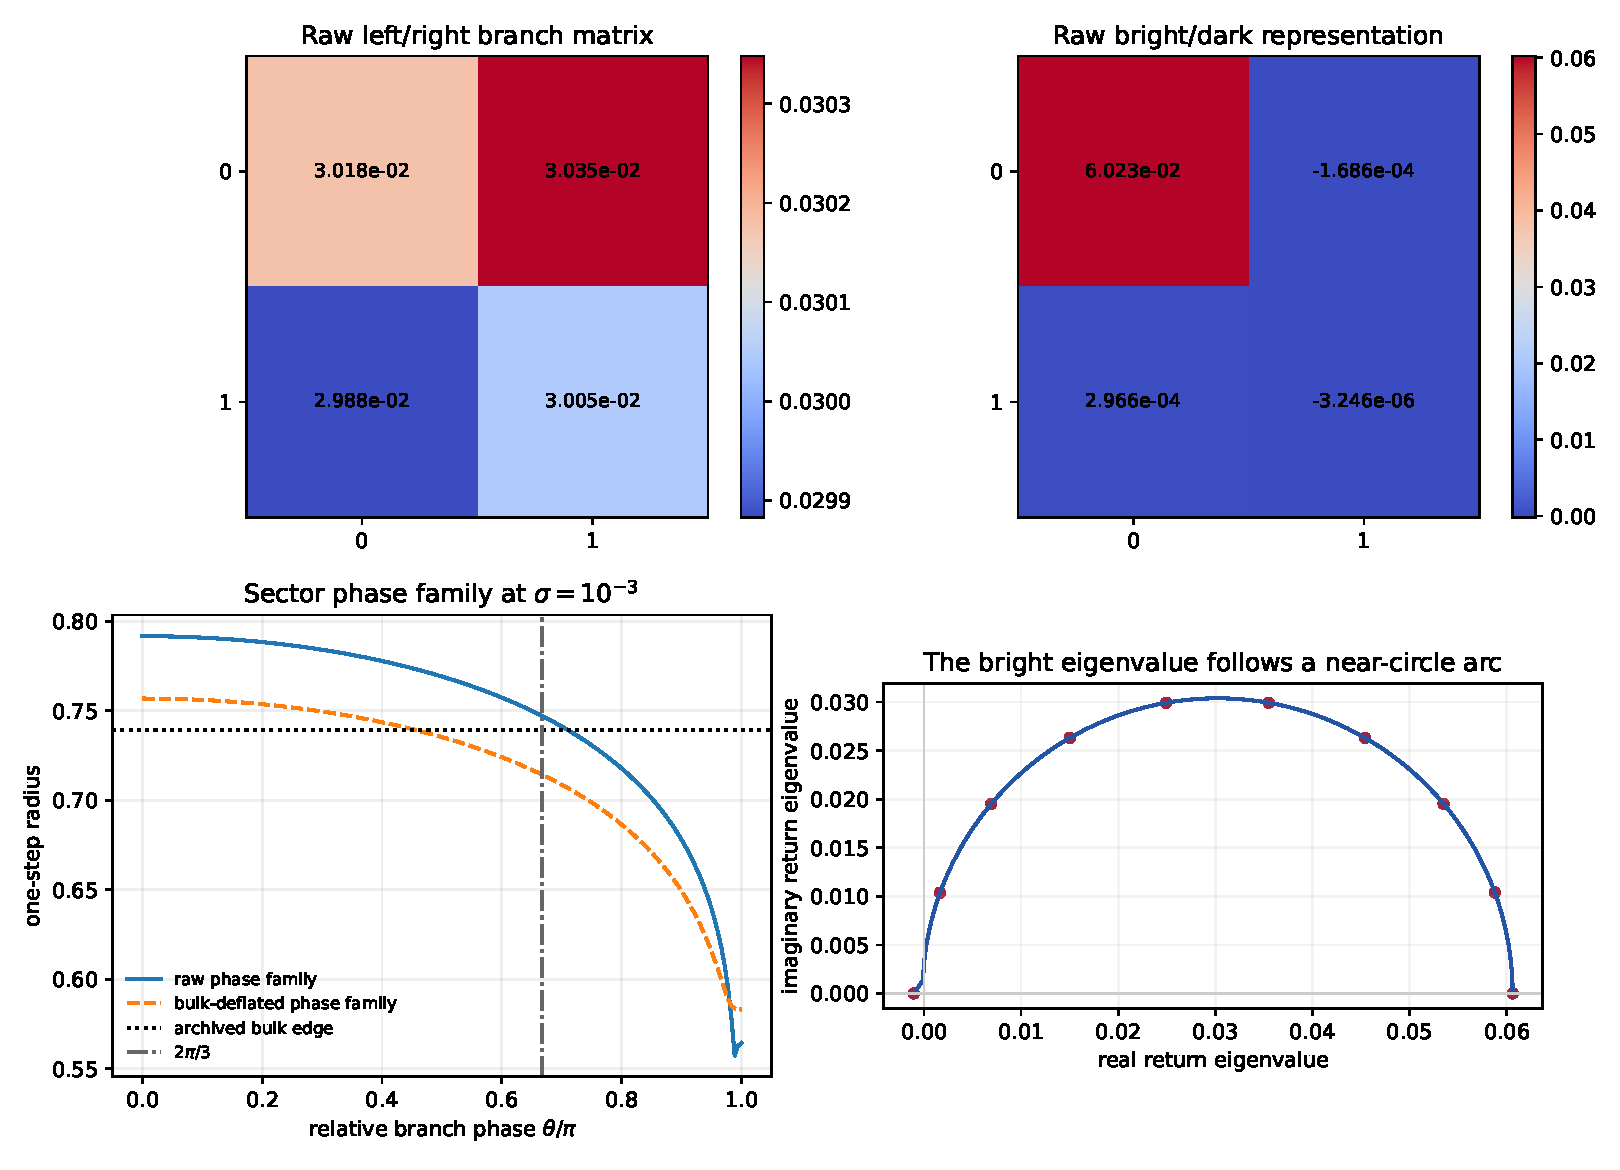
\includegraphics[width=0.9\textwidth]{figures/sector_phase_family.pdf}
\caption{Dense phase-family audit at $\sigma=10^{-3}$.  Top: the raw
two-profile matrix and its bright/dark representation.  Bottom left: raw and
bulk-deflated one-step radii as the relative branch phase varies; the dotted
horizontal line is the archived bulk edge.  Bottom right: the raw leading
return eigenvalue follows a near-circular arc, as predicted by the rank-one
formula.  The switch near $\theta=\pi$ reflects competing small eigenvalues
of a non-normal return.}
\label{fig:dense-family}
\end{figure}

\section{Discussion}
\label{sec:discussion}

\subsection{What has advanced}

The two critical branches are no longer treated as an uncontrolled scalar
complement.  They form an exact direct-sum channel, and the endpoint return
can be moved to that channel without changing its nonzero determinant.  In
the numerically dominant rank-one sector, the factor-of-two positive return,
the dark antisymmetric mode, and the effect of a relative phase are all
described by one scalar formula.

The cubic phase is therefore not an arbitrary curve fit.  It is the unique
unit-modulus relative phase that preserves one-branch amplitude in the
exchange-symmetric rank-one model.  The smallest-noise data approach both
the required branch symmetry and the predicted angle.  This is enough to
justify testing the mechanism in a derived effective Hamiltonian.

\subsection{What has not advanced}

The present calculation does not identify the branch phase of the physical
Gaussian operator.  It does not prove full-return rank-one convergence, a
uniform complement resolvent estimate, or a one-to-one correspondence
between local roots and distinct physical eigenvalues.  The dense deflated
benchmark shows why those statements cannot be inferred from the raw phase
family.

The non-identifiability proposition is equally important.  A half-weighted
positive sum reproduces the same symmetric leading radius, so radial
agreement cannot establish a complex phase.  Angular eigenvalue data,
biorthogonal entrance/exit maps, or an exact determinant combinatorics are
needed.

\subsection{No arithmetic or self-adjoint implication}

Every operator in this paper comes from one noisy quadratic map.  The cubic
root of unity is a conditional branch-closing coefficient, not a zeta zero.
No result constructs a self-adjoint Hilbert--P\'olya operator, proves a
prime-power trace formula, identifies the Riemann zeros, or implies the
Riemann hypothesis.  Any future arithmetic comparison would require an
independent trace identity not present here.

\section{Conclusion}

The branch-resolved correction survives the RH-19 no-go test in a precise
but conditional form.  Endpoint and branch returns are linked by an exact
Sylvester factorization, so the corrected two-channel determinant is
canonical.  A one-profile rank-one reduction has a bright symmetric mode
and a dark antisymmetric mode; its phase-dependent eigenvalue is
$\eta_-+e^{i\theta}\eta_+$.

If the branch weights are constrained to have unit modulus, exact branch
equivalence forces $\theta=\pm2\pi/3$ when the combined return is required to
retain one-branch modulus.  At $\sigma=10^{-4}$, both the independently
inferred phase and the archived bulk radius lie close to that conditional
prediction.  The two-profile dark/bright ratio is $1.45\times10^{-5}$.

The result is not yet a physical phase theorem.  A real half weight gives
the same symmetric radial correction, discrete time sectors do not contain
the cubic phase for general $k$, and peripheral deflation substantially
changes the dense phase family.  The next gate is therefore well defined:
derive the two branch weights from a peripherally biorthogonal,
spectral-parameter Grushin problem.  That derivation, rather than another
radial fit, will decide whether the cubic phase is a genuine mechanism or a
useful but ultimately unnecessary coordinate choice.

\section*{Data and code availability}

The source code, tests, complete CSV and JSON audits, figures, and manuscript
are available with this paper \citep{WangSectorBranchCode2026}.

\bibliographystyle{plainnat}
\bibliography{references}

\end{document}
